%# -*- coding: utf-8-unix -*-
%%==================================================
%% chapter02.tex for SJTU Master Thesis
%%==================================================

\chapter{Shuffle的优化策略}
\label{chap:optimization}

本章将详细阐述实现shuffle优化的方法论,并且依据这些方法整合形成具体优化系统---SCache。
首先SCache通过shuffle数据内存拷贝的方式来实现shuffle在计算任务中的解耦。
其次SCache通过对shuffle结合应用上下文的外部管理,并且提供shuffle读写的API,实现了一个跨平台的通用优化方案。
然后SCache通过两个启发式算法来实现对于shuffle依赖的预调度和数据预取,从而实现shuffle传输时间的优化。
此外SCache通过结合应用上下文的内存管理,来给shuffle数据提供高效的内存缓存,加速读写。
最后SCache结合网络层的优化策略为shuffle网络传输过程带来的进一步加速。

\section{Shuffle的解耦合}

要将shuffle从DAG计算任务中解耦,需要同时解决shuffle与map任务以及reduce任务的紧耦合。

在map任务完成计算之后,会产生一个键值对的集合,表示该任务计算的输出结果。
之后map任务则会根据用户定义的分区函数(比如哈希,排序等)来对这些键值对进行分块存储。
其中每一个数据块存储的是下一个reduce阶段其中一个任务的部分输入数据。
在进行分块的过程中,这些键值对就会被map任务写入到磁盘相应的文件中。
以上过程就是shuffle在map阶段的磁盘写操作,也就是图\ref{fig:workflow}中的“shuffle write”部分。
结合图\ref{fig:util}可以发现,在进行这部分操作时,并不需要大量的CPU资源。
而且由于计算已经完成,分配给该任务的slot中计算资源部分也应当在磁盘写操作之前被释放。
因此为了实现更细粒度的硬件资源管理,必须将这部分I/O操作从计算任务中解耦出来。
为了实现该部分的解耦,SCache采用了内存拷贝的技术,
即通过修改分布式DAG计算框架的部分代码,使得map任务在进行键值对分区结束后,通过内存拷贝将分区好的数据块移动到SCache的内存空间。
而在内存拷贝完成之后,该任务的slot就会被立即释放。

在reduce阶段,每一个任务开始之前,都会通过网络从远程节点的磁盘中读取该任务需要的shffle数据块,也就是图\ref{fig:workflow}中的“shuffle read”部分。
与map任务相似,在执行shuffle数据拉取的过程中,CPU资源将会被闲置。
但是与map任务不同的是,由于shuffle数据的读取是在任务开始之前,所以要优化这部分开销,就需要提前读取远程的shuffle数据到本地节点,也就是shuffle数据的预取。
为了实现shuffle数据的预取,SCache会根据任务预调度的结果,在map阶段就开始shuffle数据的网络传输。
与此同时,SCache结合DAG计算框架的任务调度信息来对预取的shuffle数据提前进行内存缓存。
与map任务类似,当reduce任务开始执行时,可以通过调用SCache的API来实现以内存拷贝的方式从本地读取shuffle数据。

通过以上方法,SCache将shuffle相关的I/O操作从map任务与reduce任务两端都进行了解耦合,将I/O资源的管理从DAG计算框架原本粗粒度的slot中进行分离,实现了更细粒度的硬件资源分配管理。
而DAG计算框架仅仅需要完成计算密集型任务与计算资源的调度管理,从而提升硬件资源利用率和复用率。

\section{结合上下文的任务预调度}

在上一小节中,我们提到了为了解耦reduce阶段的I/O操作,首先必须实现对shuffle数据的预取。
而shuffle数据与reduce任务是一一对应关系,当reduce任务被分布式DAG计算框架调度到某个节点之前,shuffle预取的目的节点也是未知的。
因此要实现shuffle数据的预取,首先需要实现对reduce任务的预调度。

在目前的DAG计算框架当中,Hadoop MapReduce通过slow-start\cite{hadoop}的方案来实现了reduce任务在map阶段的预调度,即当reduce任务被slow-start机制预调度之后,它便会占用一个slot并启动任务,开始读取shuffle远程数据。
这种预调度存在的最大问题就是会占用部分计算的资源(slot),进而影响当前未完成的map阶段的任务执行。
为了解决这个困境,SCache提出了一种辅助调度的策略。
即在map阶段,SCache通过上下文信息和map任务执行的中间状态对reduce任务进行预调度。
这轮预调度只会产生一个reduce任务与节点的映射关系,从而使shuffle数据预取成为可能。
而slot在这一轮预调度中并不会被预调度的reduce任务占用,从而避免影响map阶段的性能。
与此同时,当map阶段执行结束,分布式DAG计算框架开始调度reduce任务时,可以通过相应接口访问SCache的调度器,从而获取相应的预调度结果。
通过这种协同调度的方式,SCache实现了预调度但是不占用计算资源的任务辅助调度机制,从而解决了由于reduce任务与节点的映射未知而无法进行shuffle数据预取的困境。

\subsection{随机任务预调度的问题}

实现任务预调度最简单的方式便是随机均匀地将下一阶段的任务分配到各个计算节点上。
虽然这种简单的随机调度能保证各个节点在任务数目上的均衡,但是真正的负载并不仅取决于任务数目,也需要考虑每个任务所需要计算的数据量。
在图\ref{fig:sim}中我们展现了使用OpenCloud\footnote{http://ftp.pdl.cmu.edu/pub/datasets/hla/dataset.html}公开的任务运行日志对不同任务预调度算法的性能测试。
在这里我们比较了三种不同的调度算法在调度不同轮次的任务时性能,包括随机调度算法,Spark默认调度算法(First-In-First-Out,FIFO)\cite{apachespark}以及我们提出的基于启发式的最小堆算法。
图\ref{fig:sim}中的红色点状线段为比较基准线,通过计算在Spark默认调度算法下的计算阶段完成时间来获得。
然后我们假设在shuffle数据已经获得预取的情况下,移除了日志中shuffle读取的时间开销,然后比较了以上三个算法对于基准线的性能变化。
需要注意的是在OpenCloud公开的日志中,大部分应用都只包含了少量的shuffle开销。
图\ref{fig:cdf}展现了在OpenCloud日志中shuffle传输时间占整个reduce计算阶段完成时间比例的累积分布。
其平均shuffle传输时间只占到了reduce阶段完成时间的3.2\%。

\begin{figure}[!htp]
    \centering
	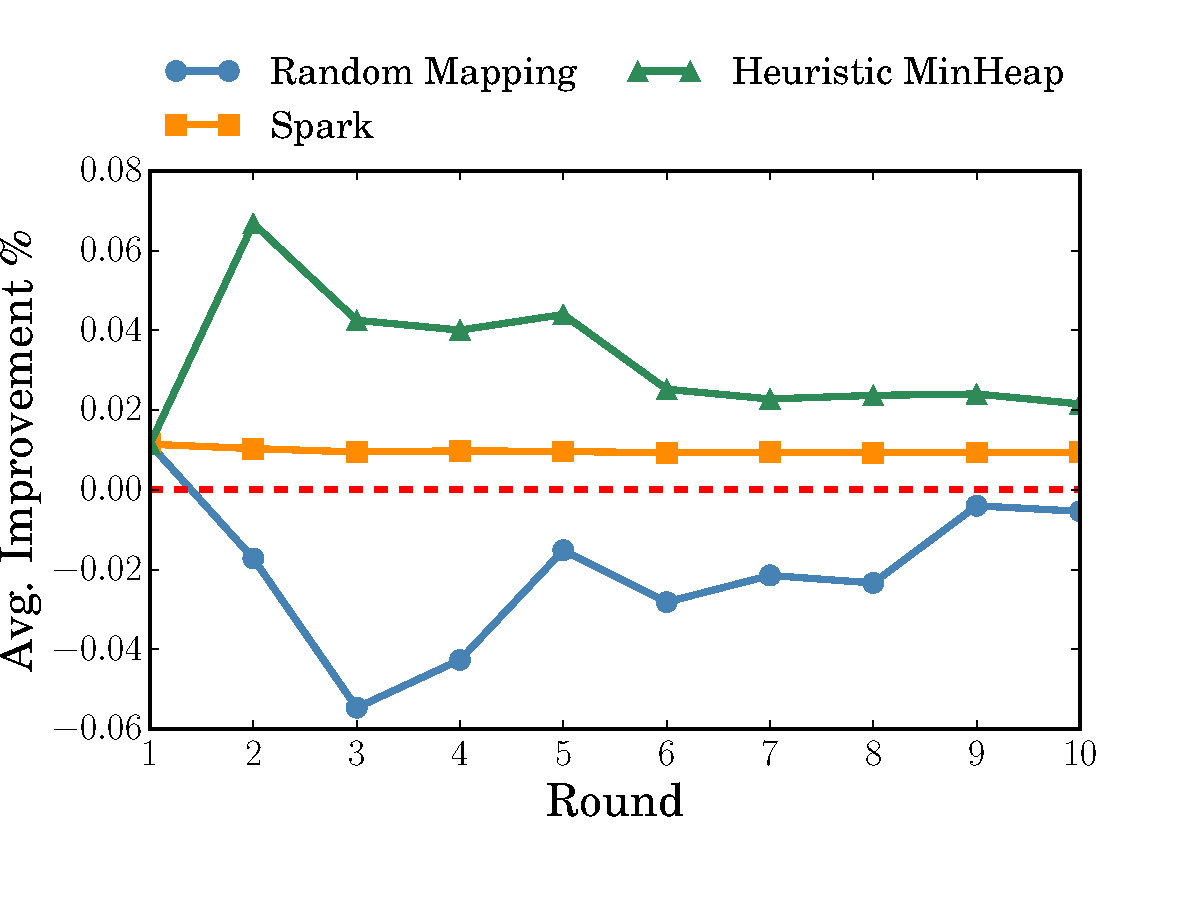
\includegraphics[width=0.7\textwidth]{../../PPoPP-2018/fig/sim.pdf}
	\bicaption[fig:sim]{基于OpenCloud日志的计算阶段完成时间提升}{基于OpenCloud日志的计算阶段完成时间提升}{Fig}{Stage Completion Time Improvement of OpenCloud Trace}
\end{figure}

\begin{figure}[!htp]
    \centering
	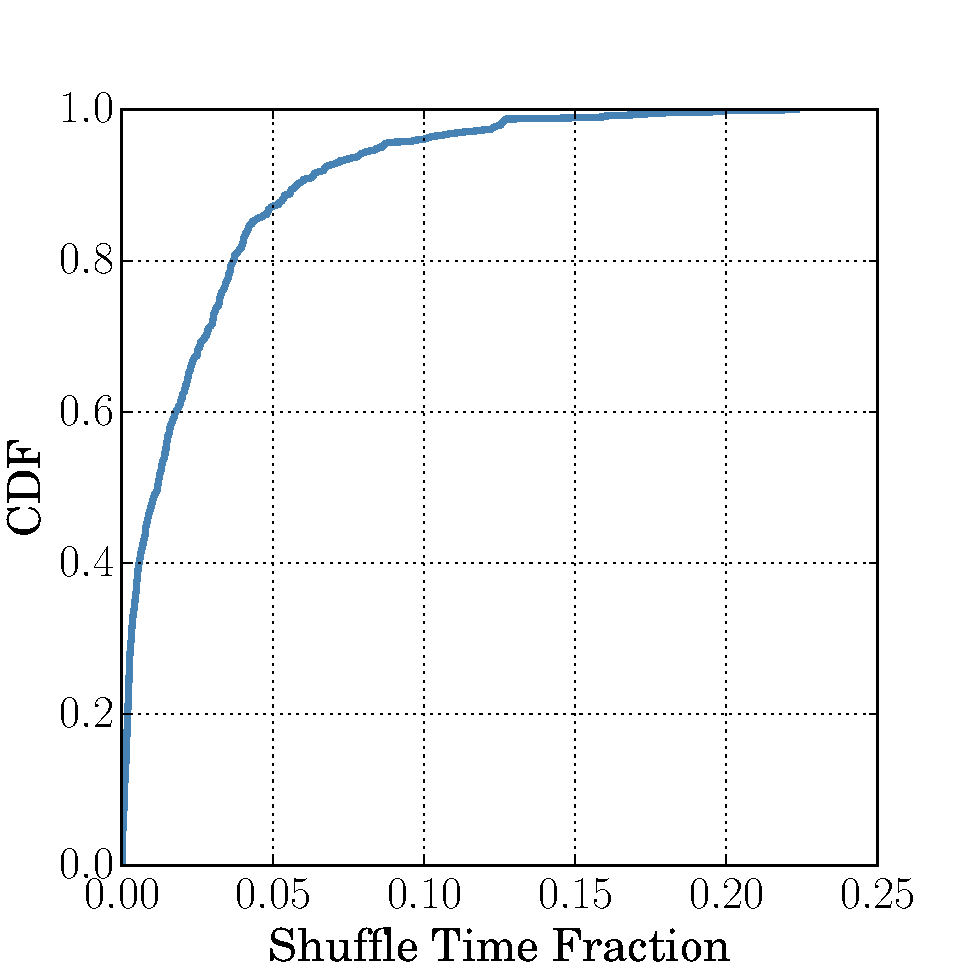
\includegraphics[width=0.6\textwidth]{../../PPoPP-2018/fig/reduce_cdf.pdf}
	\bicaption[fig:cdf]{OpenCloud日志中shuffle时间占比累积分布}{OpenCloud日志中shuffle时间占比累积分布}{Fig}{Shuffle Time Fraction CDF of OpenCloud Trace}
\end{figure}

虽然这是一个相对轻量shuffle的工作日志,但是在模拟中我们发现随机调度算法仅仅只能在只有一轮计算任务的情况下获得一个较好的性能提升。
随着任务执行轮次的增加,随机调度算法的性能甚至不如没有经过shuffle预取优化的基准线。
究其原因,是由于在分布式DAG计算过程当中,普遍存在数据分区之后体积的分布不均的现象,即数据倾斜(data skew)\cite{reining, gufler2012load, skewtune}。
在随机调度算法中,可能会把几个输入数据相对较大的任务调度到一个节点上。
因为受限于BSP的同步模式,一个计算阶段的完成需要等到该阶段所有任务的完成。
这种缓慢任务的碰撞会拖慢整个计算阶段的完成,进而使得性能甚至不如没有优化的基准线。
此外,随机调度完全忽略了shuffle数据的本地性,因而可能在shuffle网络传输阶段引入额外的流量开销。

\subsection{预测shuffle数据分布}

随机任务预调度之所以会造成这些问题是因为其算法只考虑了在任务数上的均匀分配,而没有考虑每个任务本身的负载,也就是其计算所需要的输入数据体积。
同时,随机任务调度在调度过程中完全忽略了应用的上下文信息,比如map阶段产生的shuffle数据的体积分布等。
而一个较优的调度结果可以在已知:1)reduce计算阶段总共依赖的shuffle数目,2)该reduce阶段的任务数目(即shuffle数据块个数)以及3)每个shuffle中数据块体积,这些参数的情况下做出。
在这些都已知的情况下,对于每个reduce任务计算所需要的输入数据体积就能够被计算出来。
如果不考虑数据本地性,则该调度问题可以被转化为经典的makespan问题,通过近似算法可以获得至少2倍于最优值的调度结果\cite{approximation}。
而这三个参数中,对于reduce计算阶段的shuffle依赖数目以及该阶段的任务数目都可以通过提取DAG计算框架中的应用信息来获取。
比如Spark在生成RDD的转换关系的同时,就可以获取这两者的信息\cite{spark}。
在此基础上,如果可以对shuffle数据的体积分布进行相对准确的预测,那么就可以基于此做出一个较优的预调度结果。

\begin{figure}[!htp]
	\centering
	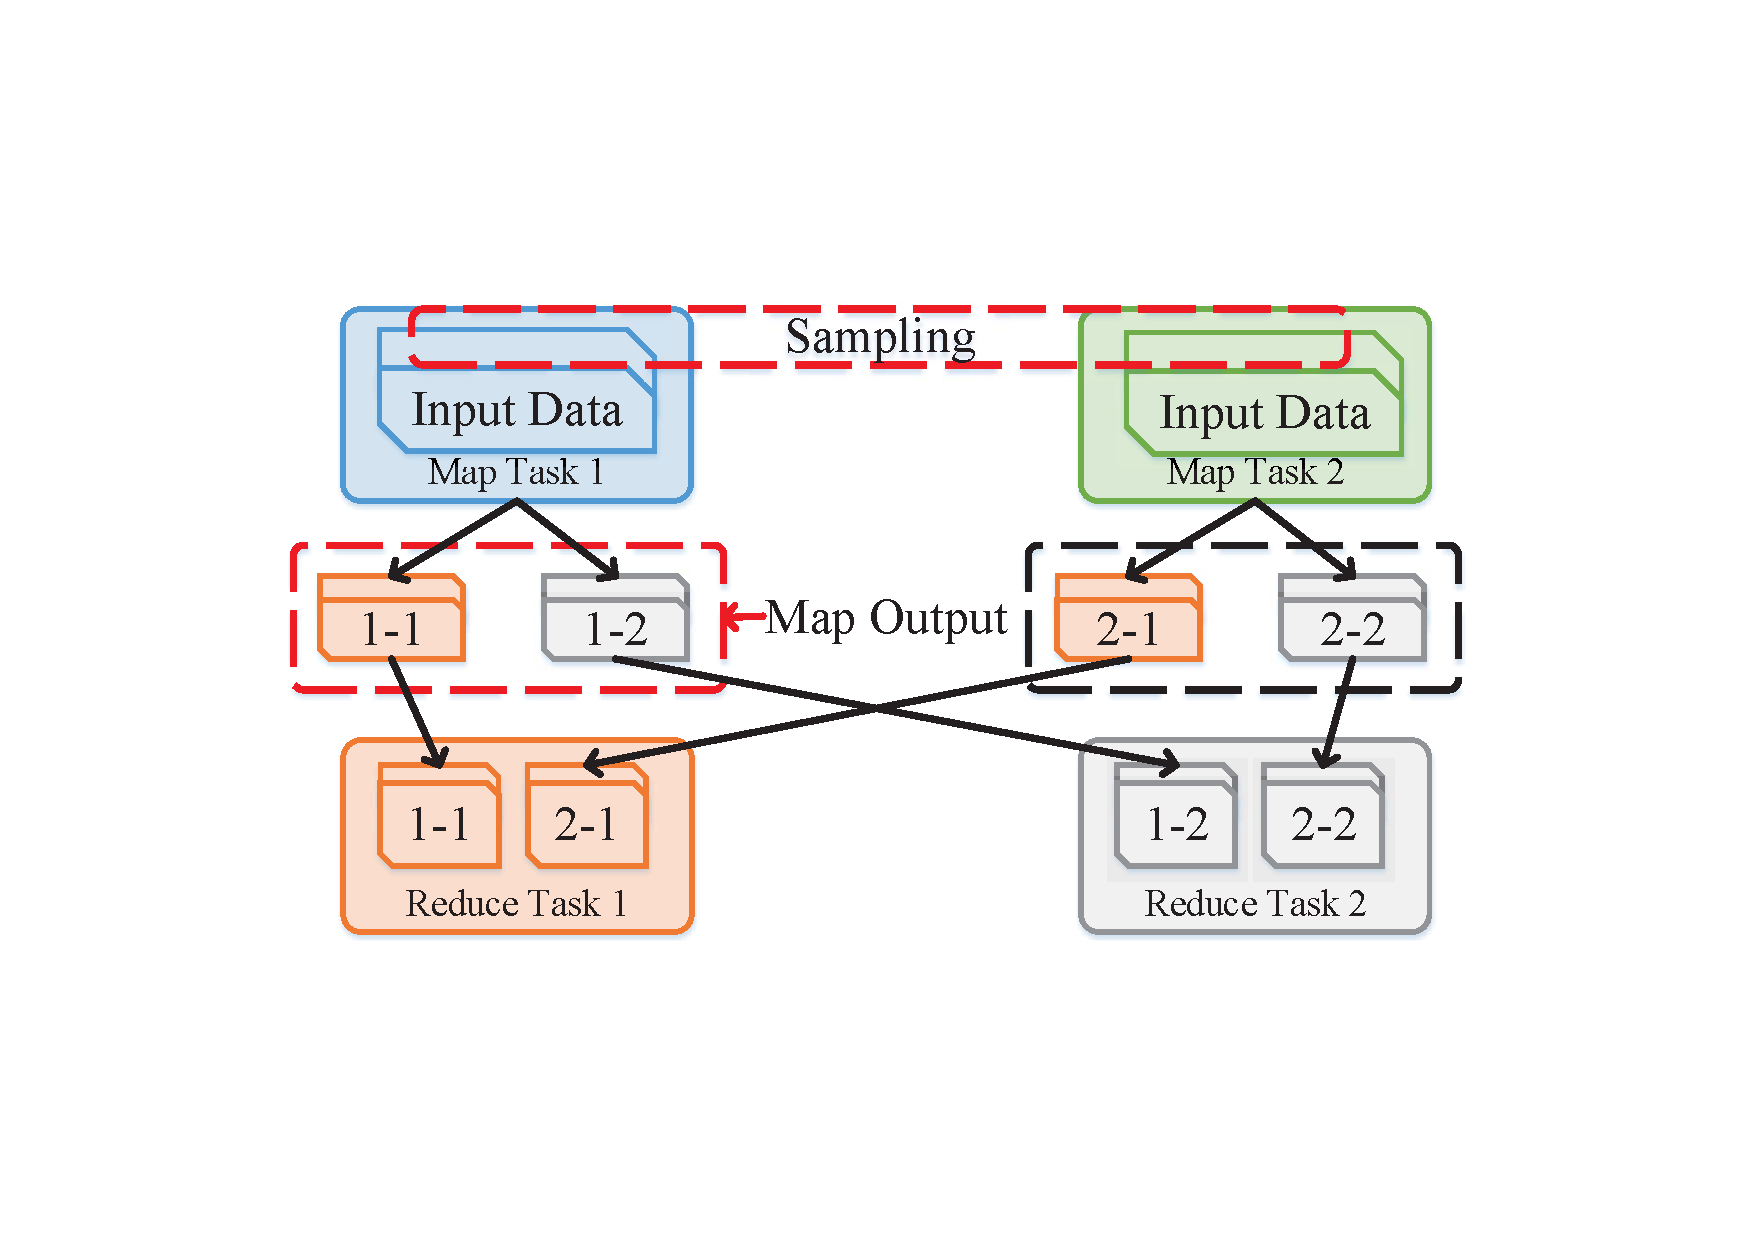
\includegraphics[width=0.6\textwidth]{../../PPoPP-2018/fig/shuffle.pdf}
	\bicaption[fig:shuffle]{Shuffle数据分布预测示意图}{Shuffle数据分布预测示意图}{Fig}{Shuffle Data Prediction}
\end{figure}

如图\ref{fig:shuffle}所示,根据DAG的计算流程,每一个reduce任务需要获取的shuffle数据取决于:上一阶段每个map任务的输入数据体积和map任务的计算过程和用户定义的分区函数。
对于map阶段的每一个计算任务,都会产生一个对应于reduce阶段某一个任务的数据块。
因此reduce阶段一个任务的输入数据体积大小$reduceSize_i = \sum_{j=0}^{m} {BlockSize_{ji}}$,其中$m$代表map阶段任务的数目。
$BlockSize_{ji}$代表了这个数据块是由第$j$个map任务产生,属于第$i$个reduce任务的输入(比如图\ref{fig:shuffle}中数据块“1-1”)。
本文将$BlockSize_{ji}$代表的体积分布成为shuffle数据的分布。

对于一些DAG较为简单的应用,比如Hadoop MapReduce中的工作\cite{hadoop},由于reduce阶段的shuffle的依赖往往只有一个,因此对于shuffle数据分布的预测就相对容易。
许多研究工作证明,对于此类工作,在执行工作的配置没有改变的情况下,上文所提到的$BlockSize_{ji}$可以通过简单的线性回归模型获取比较高的预测精度\cite{ishuffle, predict}。
这种线性回归模型采用了对已经运行结束的map任务产生的shuffle数据块进行统计,获取当前这些数据块中属于不同reduce任务的体积,然后采用线性回归的方法,结合剩余map任务的个数以及其相应的输入数据来对shuffle的数据分布做出预测,最终获得reduce阶段任务输入数据的体积分布。

但是随着分布式DAG计算框架的演化,计算逻辑的表达和数据依赖关系变得日趋复杂。这些计算过程中的不确定性都会影响到shuffle数据的预测精度。
比如在Spark中一个由用户自定义的数据分区函数就有可能会使当前已经获取的map任务产生的shuffle数据分布与最终的shuffle数据分布产生巨大的不一致性。
\begin{figure}[!htp]
    \centering
    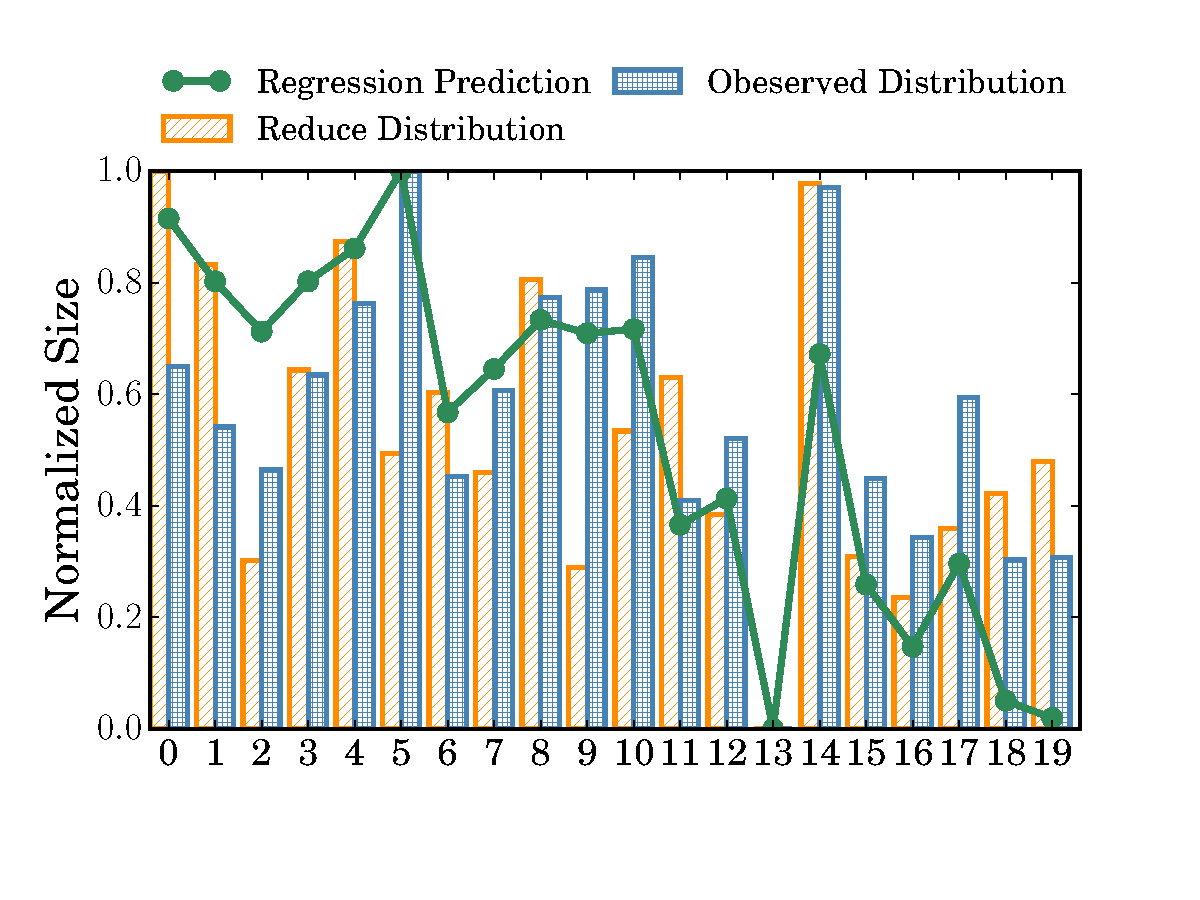
\includegraphics[width=0.6\textwidth]{../../PPoPP-2018/fig/hash_pre.pdf}
	\bicaption[fig:hash_pre]{哈希分区函数下线性回归预测结果}{哈希分区函数下线性回归预测结果}{Fig}{Linear Regression Prediction of Hash Partitioner}
\end{figure}

为了更直观地展示这种不一致性,我们对不同的数据集在不同分区函数情况下应用线性回归模型预测的结果进行了测试。
这两种数据集都被划分成20个分块,并且通过一次map阶段计算后经由不同的分区函数进行分区,其对应的reduce分区数目也是20。
在图\ref{fig:hash_pre}中,展示了在哈希分区函数对随机数据集进行分区的情况下,线性回归模型的预测情况。
图\ref{fig:range_pre_sample}则展示了在数据本地性倾斜度较高的数据集中使用范围分区函数进行数据分块的情况下,线性回归模型和采样预测的情况。
图\ref{fig:prediction_relative_error}则表示在使用与图\ref{fig:range_pre_sample}同样的数据集与分区函数的情况下,线性回归模型与采样预测结果的相对真实数据误差。

由于本文的两个预测方法均用来预测reduce任务输入数据的体积分布,而不需要预测绝对体积,因此为了方便比较,以上图中所有数据都被标准化到0-1之间。
图\ref{fig:hash_pre}和图\ref{fig:range_pre_sample}中“Observed Distribution”表示在我们随机选取的几个map任务中,这些任务的shuffle结果对应于各个reduce任务的数据总和的分布。

\begin{figure}[!htp]
    \centering
	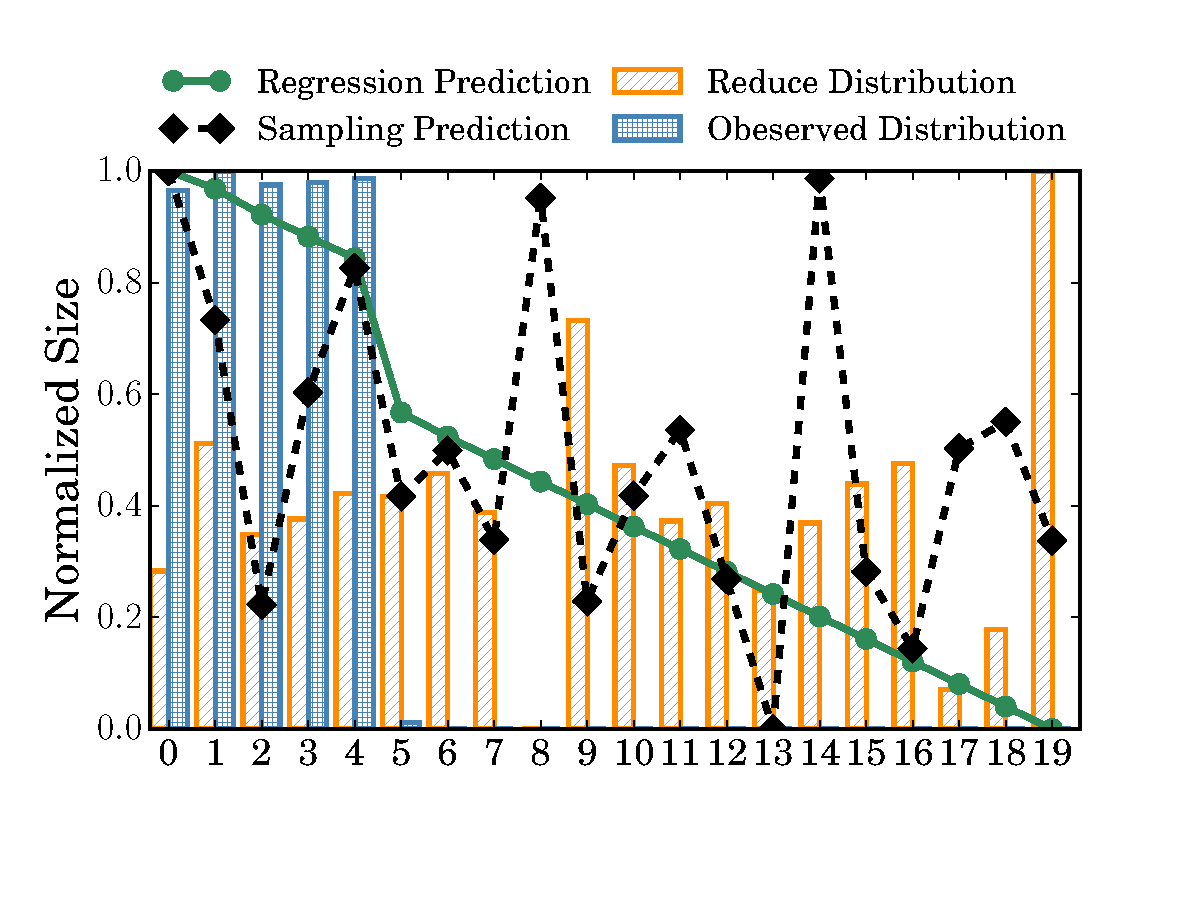
\includegraphics[width=0.6\textwidth]{../../PPoPP-2018/fig/range_pre_sample.pdf}
	\bicaption[fig:range_pre_sample]{范围分区函数下线性回归预测与采样预测的结果}{范围分区函数下线性回归预测与采样预测的结果}{Fig}{Linear Regression and Sampling Prediction of Range Partitioner}
\end{figure}

\begin{figure}[!htp]
    \centering
	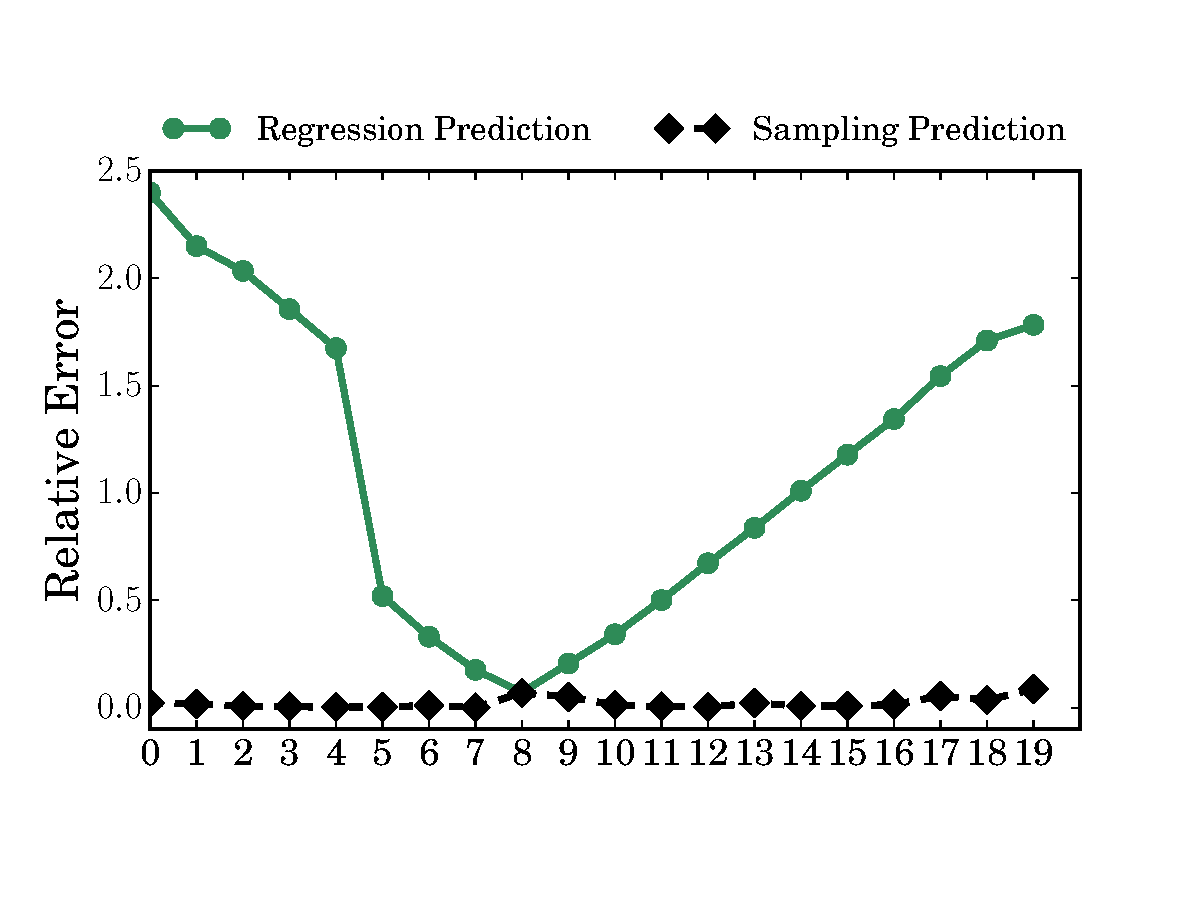
\includegraphics[width=0.6\textwidth]{../../PPoPP-2018/fig/prediction_relative_error.pdf}
	\bicaption[fig:prediction_relative_error]{范围分区函数下不同预测方法的相对误差}{范围分区函数下不同预测方法的相对误差}{Fig}{Prediction Relative Error of Range Partitioner}
\end{figure}

可以看到在图\ref{fig:hash_pre}中,因为预测对象是基于随机数据集和哈希分区函数,所以在“Observed Distribution”中观测到的下阶段每个reduce任务的数据体积与最终真实的数据体积分布比较接近。
因此,依据这些观测到的一部分shuffle数据的分布来对reduce任务的最终输入数据分布做一个线性回归的预测具有较高的准确性。
但是当遇到数据本地性倾斜时,由于当前观测的数据分布代表性不足,使得线性回归在这种情况下会产生巨大的偏差。
图\ref{fig:range_pre_sample}就是一个极端的例子,可以看到在图中由于当前选取的几个map任务产生的shuffle数据中缺乏5-20的reduce任务数据,因此使线性回归预测在这里产生了巨大误差。

为了防止这种情况的发生,我们提出了一种基于水塘抽样算法(Reservoir Sampling)\cite{reservoir}的采样预测方案来缓解数据本地性倾斜带来的预测偏差。
这里我们对水塘抽样算法做出了改进,对于每一个抽样的map任务数据,我们依据其体积大小赋予了样本不同的权重。
在对上文提到的$BlockSize_{ji}$:
\begin{equation}
	\label{eq:sample}
	BlockSize_{ji} = {{InputSize_j \times \frac{sample_i}{s \times p}}} \quad (sample_i =  \text{number of samples for }reduce_i)
\end{equation}
如图\ref{fig:shuffle}中的“Sampling”所示,对于map阶段的每个任务的数据块,我们采用经典的水塘抽样算法随机选取$s \times p$个样本,其中$p$表示下一个reduce阶段的任务数目,$s$是一个可以配置的参数。
采样结束后,map阶段的本地计算任务就会被启动,用来对采样数据进行计算和分区,最终可以获得该map任务对于下阶段$reduce_i$产生的数据量,也就是$sample_i$。
当每个节点完成本地的采样之后,这些数据会被汇总到中心调度器上进行汇总,而每个map任务对应的数据块体积大小则被作为权重来获得最终的预测分布。

\begin{figure}[!htp]
    \centering
    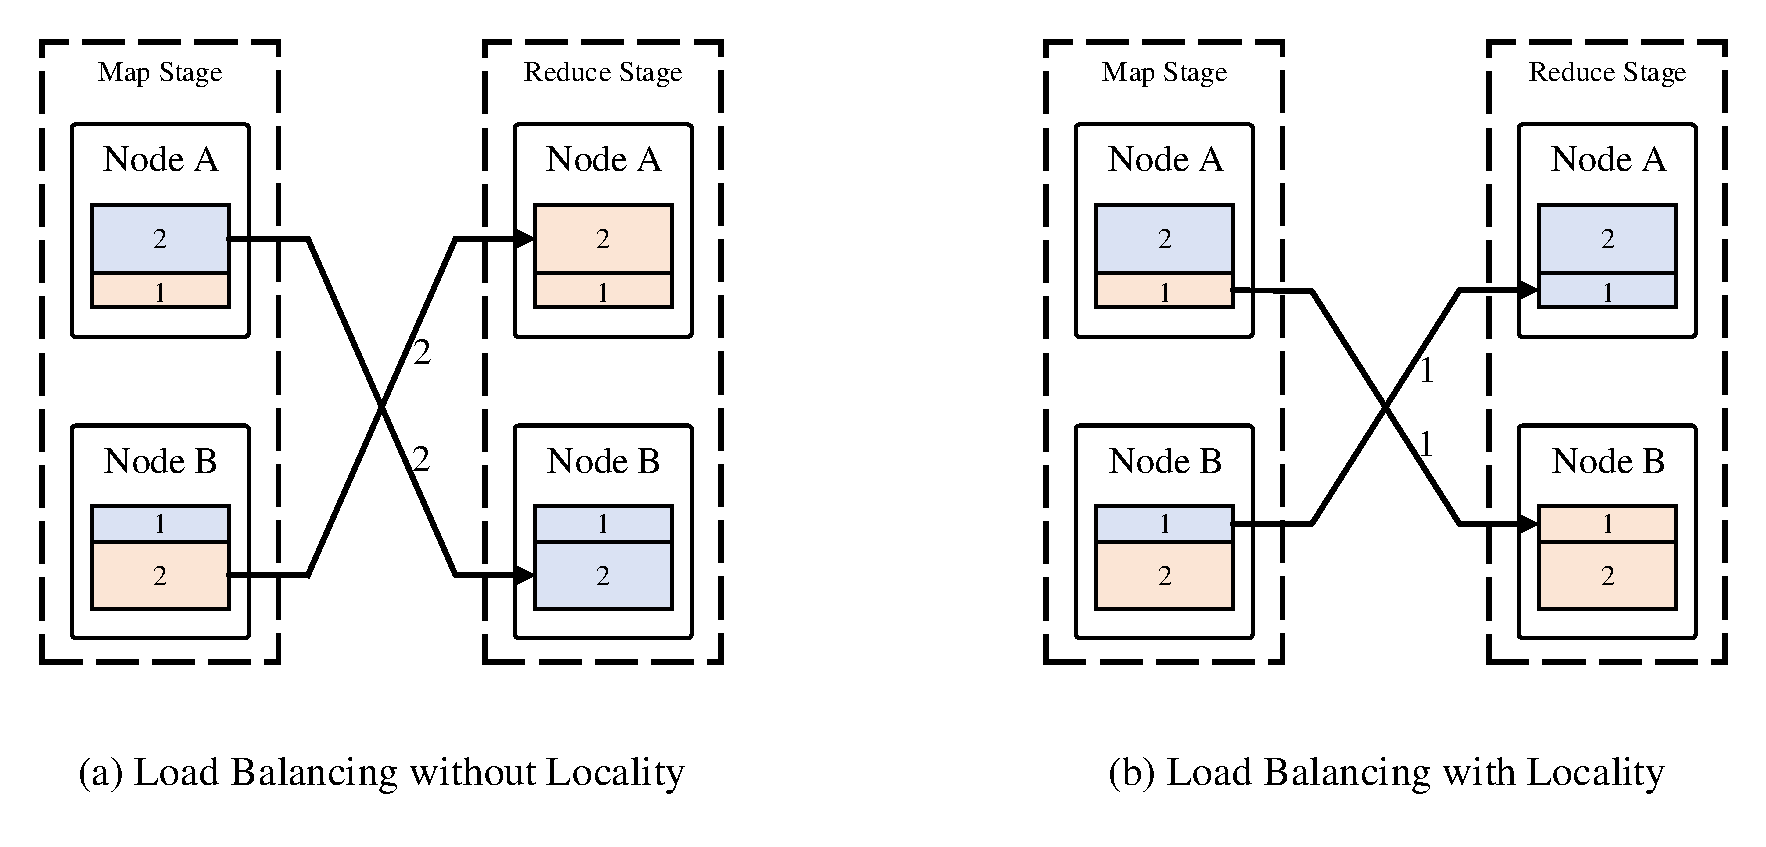
\includegraphics[width=0.8\textwidth]{locality.pdf}
	\bicaption[fig:locality]{Reduce任务负载均衡调度中的数据本地性}{Reduce任务负载均衡调度中的数据本地性}{Fig}{The Data Locality in Reduce Tasks Load-Balanced Scheduling}
\end{figure}

在图\ref{fig:range_pre_sample}中,我们将$s$设置为3。
可以看到相较于线性回归模型,采样预测的精度即使在数据具有极端本地性倾斜的场景中也能获得比较不错的结果。
需要注意的是,图中采样预测的分布曲线与最终真实数据的分布曲线在标准化之后并不是完美匹配的。
产生这种波动的原因是该数据样本在shuffle过程中虽然存在严重数据本地性倾斜,但是由于其最终的reduce分布的绝对体积较为接近,因此使得预测结果的波动在标准化到0-1区间之后被放大。
在本次预测过程当中,预测结果的数值的整体标准差只有0.0015。
为了进一步说明采样预测的有效性,我们在图\ref{fig:prediction_relative_error}中从预测的绝对体积上比较了两种方法在数据极度本地性倾斜下的表现。
我们将真实的reduce任务数据体积作为基准,比较不同预测方案得出的每个reduce任务的体积与真实值的相对误差。
可以发现,采样预测甚至可以在数据体积的绝对值上接近与真实值。
而相反线性回归模型在这种极端情况下表现就很差。

虽然采样预测能够提供非常好的精确性,但是由于需要在本地对小部分数据进行map阶段的任务计算,因此也会带来额外开销。
为了避免这种额外开销,采样预测只有在一些容易产生数据本地性倾斜的分区函数时才会被触发,比如范围分区函数,用户自定义的分区函数等。
对于采样预测带来的开销,我们将在章节\ref{chap:evaluation}中做出详细的测试。
在对shuffle的数据做出预测的同时,考虑到数据本地性的特征,我们还会对每个reduce任务的输入数据中的所有数据来源做一个计算,并算出该数据块中来源最高的数据块的占比。
即:
\begin{equation}
	\label{eq:prob}
	prob_i = \max_{0 \leq j \leq m} \frac{BlockSize_{ji}}{reduceSize_i} \quad (m = \text{number of map tasks})
\end{equation}
这个参数用来表示当该reduce任务被调度到产生$prob_i$这部分数据所在的节点时,将获得最小的通过网络传输的shuffle数据量,即最好的本地性。
在接下来的算法中,该参数也会作为提高shuffle效率的一部分因素来影响调度的最终结果。

\subsection{启发式预调度}
\label{subsec:schedule}

当取得对于reduce任务的输入数据预测结果之后,就需要对这些任务进行预调度,从而实现shuffle数据的预取。
如果不考虑本地性,那么任务的调度只需要根据预测结果做出一个负载相对均衡的方案即可。
而这种任务到节点的调度问题在不考虑本地性的情况下可以转化成经典的makespan问题,从而通过近似算法求得一个较优解\cite{approximation}。
这些近似算法已经被证明至少不会差于最优解的2倍。
但是如果考虑到数据本地性,使得任务完成时间仅仅依靠数据大小这个关联被打破。
因为存在两种负载相同的调度,由于本地性的不同使得网络数据传输量不同,那么对于数据传输量较大的方案,即本地性较差的调度方案,其任务完成时间受到网络传输延迟的影响的可能性就更大。
比如图\ref{fig:locality}中,两个节点在reduce阶段分别需要运行一个体积为3的reduce任务,图中(a)和(b)的调度方案最终A,B节点的负载都是一致的。
但是如果不考虑数据本地性,即如\ref{fig:locality}(a)中的调度方案,那么网络中需要传输的shuffle数据体积便是4。
而如果考虑到数据本地性,那么最优的调度方案应如图\ref{fig:locality}中(b)所示。
图\ref{fig:locality}在保证reduce阶段各个节点负载均衡的情况下使得shuffle的传输量下降到了2。

\begin{figure}[!htp]
    \centering
    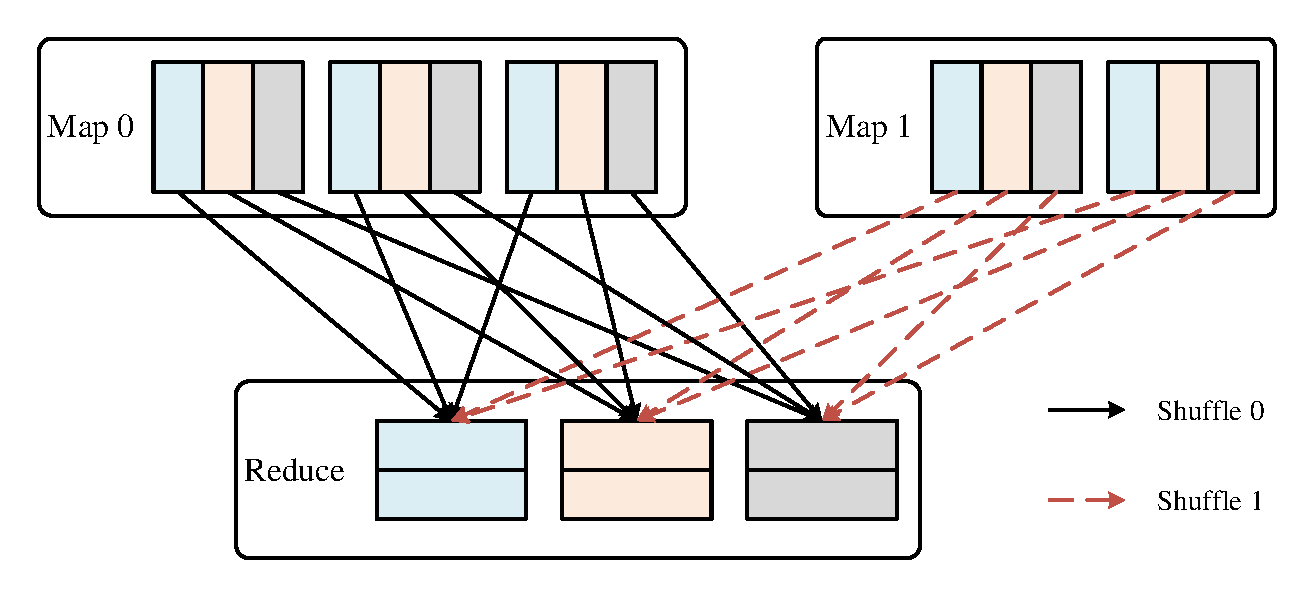
\includegraphics[width=0.8\textwidth]{../figure/twoshuffles.pdf}
	\bicaption[fig:twoshuffles]{多shuffle依赖}{多shuffle依赖}{Fig}{Multiple Shuffle Dependencies}
\end{figure}

考虑数据本地性可以获得更好的调度结果,但也使得本身就是NP难的负载均衡调度问题变得更加复杂。
为了解决这个问题,我们提出了一个综合考虑本地性以及负载均衡的启发式算法来针对单个shuffle依赖的reduce阶段的任务进行预调度(Heuristic MinHeap算法\ref{hminheap})。
对单个shuffle依赖的启发式调度算法主要可以分为两轮的调度。
在第一轮调度中(即算法\ref{hminheap}中的第一个while循环),算法首先根据对reduce任务数据体积的预测结果将其进行按体积降序排序。
同时,我们采用了一个最小堆来维护集群中的节点,这个最小堆的排序比较依据便是调度到该节点上的所有任务体积之和。
经过这一轮调度之后,一些输入数据体积较大的reduce任务将会被均匀的分散调度到不同节点上,同时尽量保证了各个节点之间的负载均衡。
在第二轮的调度中,算法会根据数据本地性这个属性来对第一轮已经完成的任务---节点映射关系做出调整。
算法中的$SWAP\_TASK$函数只有在任务当前分配的节点(算法中$assign\_id$)与数据本地性最好的节点(算法中的$host\_id$)不匹配时才会被触发。
对于一个shuffle数据最多有$prob$比例来自于$host$的reduce任务,算法通过标准化计算出了$norm$作为该任务可以用来换取数据本地性的性能开销极大值。
这个标准化计算使得任务在用牺牲性能换取更好的本地性的同时,不会让性能的损失超过原先该reduce计算阶段的10\%。

通过启发式的任务本地性交换策略,使得该算法在保证负载均衡的同时获取一个相对较好的本地性,从而尽可能避免引入额外的网络shuffle数据传输。
即使相较于Spark原生的FIFO调度策略\cite{sparksource},本算法在负载和数据本地性上都能获得更优的效果。
我们同样使用了OpenCloud的公开日志作为输入测试了该算法的效果。
如图\ref{fig:sim}中“Heuristic MinHeap”的曲线所示,本算法可以获得相较于Spark原生算法更好的性能提升。
相较于Spark调度算法平均2.7\%的性能提升,算法\ref{hminheap}平均可以获得5.7\%的性能提升。
这个更均匀的负载与更好的本地性也是在基于应用上下文的情况下对shuffle数据做出预测后的调度所获得的一个附加的优势。

\subsection{处理多shuffle的依赖}

在目前大数据应用日益复杂的前提下,分布式DAG计算框架也相应的提供了更复杂的计算逻辑支持。
而为了满足这些复杂逻辑支持,使得在DAG中一个计算阶段对多个shuffle依赖的情况广泛存在。

如图\ref{fig:twoshuffles}所示,其中展现了一个存在两个shuffle依赖的reduce计算阶段。
在单个shuffle依赖的情况下,只需要在map阶段的前期对shuffle数据进行预测即可做出reduce阶段的任务预调度与shuffle数据预取。
但是对于依赖多个shuffle的reduce阶段,其任务输入数据最终取决于所有shuffle依赖对应的map计算阶段的任务结束后的输出数据分布。
在小节\ref{subsec:schedule}中提到的方法只能解决对于单个正在执行的shuffle的数据预测与相应的任务预调度。
在多个shuffle依赖的情境中,对于没有被执行的那些shuffle依赖,因为还不存在map任务的部分执行结果,也没办法对其进行采样,因而不能对这些shuffle的数据做出预测。
其中一种解决这个困境的方案就是让分布式DAG计算框架对所有shuffle依赖的全部map阶段任务进行同时调度。
但是这么做不仅会破坏原先各个分布式DAG计算框架的设计,也会带来不可忽视的额外开销。
比如因为每个阶段map任务的逻辑不同,所以在执行器执行任务过程中,这种同时调度的方式就会带来在JVM中任务额外的序列化开销。
而目前DAG框架为了减少重复地对任务代码进行序列化,大都只采用了一个计算阶段内部任务的并行。
因此为了防止破坏这些DAG计算框架提供的优化执行方案,我们设计了一种累积的启发式调度算法(算法\ref{mhminheap})来处理对于多个shuffle依赖的reduce任务预调度。

\begin{algorithm}[H]
\caption{单shuffle依赖的启发式调度}
\label{hminheap}
	\begin{algorithmic}[1]
	\small
	\Procedure{\Large schedule}{$m, host\_ids, p\_reduces$}
		\State $m\gets$ partition number of map tasks
		\State $R\gets$ sort $p\_reduces$ by size in descending order
		\State $M\gets$ min-heap $\left\{ host\_id \rightarrow \left( \left[ reduces \right], size \right) \right\}$
		\State $idx\gets$ len$\left(R\right) - 1$
		\While{$idx \geq 0$}
		\Comment{Schedule reduces by MinHeap}
		\State $M\left[0\right].size \mathrel{+}= R\left[idx\right].size$
		\State $M\left[0\right].reduces.append\left(R\left[idx\right]\right)$
		\State $R\left[idx\right].assigned\_host \gets M \left[0\right].host\_id$
		\State Sift down $M\left[0\right]$ by $size$
		\State $idx\gets idx-1$
		\EndWhile
		\State $max\gets$ maximum size in $M$
		\State Convert $M$ to mapping $\left\{ host\_id \rightarrow \left( \left[ rid\_arr \right], size \right) \right\}$
		\ForAll{$reduce$ in $R$}
		\Comment{Heuristic swap by locality}
			\If{$reduce.assigned\_id \neq reduce.host\_id$}
				\State $p\gets reduce.prob$
				\State $norm\gets \left(p-1/m\right)/\left(1-1/m\right)/10$
				\State $upper\_bound \gets \left(1 + norm\right) \times max$
				\State SWAP\_TASKS$\left(M, reduce, upper\_bound\right)$
			\EndIf
		\EndFor
		% \Comment{$m$ is the number of input data}
		% \Comment{$r$ is partition number of reduces}
		% \Comment{$hosts$ is array of (hostid, partitionids[], size)}
		% \Comment{$c$ is $r*m$ array of composition data}
		% \Comment{$pSize$ is $r$ size array of predicted size of reduces}
		\Return $M$
	\EndProcedure
	\Procedure{\Large swap\_tasks}{$M, reduce, upper\_bound$}
		\State $reduces \gets M\left[reduce.host\_id\right].reduce$	
		\State $candidates \gets$ Select from $reduces$ that $assigned\_id \neq host\_id$ \textbf{and} total size closest to $reduce.size$
		\State $\Delta size \gets sizeOf\left(candidates\right) - reduce.size$
		\State $size\_host \gets M\left[reduce.host\_id\right].size - \Delta size$
		\State $size\_assigned \gets M\left[reduce.assigned\_id\right].size + \Delta size$
		\If{$size\_host\leq upper\_bound$ \textbf{and} \\
			\qquad \; $size\_assigned\leq upper\_bound$}
			\State Swap $candidates$ and $reduce$
			\State Update $size$ in $M$
			\State Update $assigned\_host$ in $candidates$ and $reduce$
		\EndIf
	\EndProcedure
	\end{algorithmic}
\end{algorithm}

具体过程如$M\_SCHEDULE$函数中所描述的。算法会记录经过若干轮的预调度之后,当前每个节点所积累的reduce任务数据量,即算法中的$shuffles$变量。
当一个新的shuffle依赖中的map计算阶段开始执行,$M\_SCHEDULE$就会被调用,并且根据之前调度结果的累积进行新一轮的调度。
首先算法会先将新一轮的预测shuffle数据分布与之前的累积值进行相加,从而更新每个reduce任务中($p\_reduce$)相应的$prob$值和对应的$host$。
更新之后便会调用算法\ref{hminheap}中的$SCHEDULE$函数进行新一轮的任务预调度。
而当新的预调度结果产生之后,算法就能获取一个新的任务 --- 节点的映射关系。
对于那些任务中新分配的节点($assigned\_host$)与之前一轮调度中分配的节点不同的任务,算法会触发一次网络重传,将原先已经预取到旧的节点上的数据重新传输到新分配的节点(re-shuffle)。
Re-shuffle的过程会引入额外的开销,但是由于之前若干shuffle数据预取的累积,使得相应的$prob$值也就越大,因而算法在$SWAP\_TASK$的本地性任务交换中更倾向于原节点。
因此,在累积调度过程中,算法\ref{mhminheap}不仅能保证多shuffle依赖下对reduce数据的预测,同时也能在保证负载均衡和本地性的同时将re-shuffle的开销尽可能地降低。

\section{基于应用上下文的内存管理}

在章节\ref{chap:observations}中提到了关于shuffle数据体积的观察。
虽然shuffle数据相较于应用的输入数据体积较小,而且当前用于计算的内存也日益增大,但是我们仍然需要对shuffle数据在内存中的缓存进行精细的管理,防止其过多占用内存而影响DAG计算框架的执行性能。

为了缓存数据,SCache首先需要在节点内存中占用一部分内存作为存储shuffle的专用内存空间。
当其中缓存的shuffle数据超过占用的内存体积时,需要将一部分数据先保存到硬盘上,并且在这部分数据被使用之前重新将他们放入内存中。
为了实现内存缓存对性能提升的最大化,我们在这里结合了分布式DAG计算框架调度任务的特点,提出了两条管理shuffle内存的规则:全部或者没有(all-or-noting)和基于上下文的优先级。

\begin{algorithm}[H]
	\caption{多shuffle依赖的累积启发式调度}
	\label{mhminheap}
	\begin{algorithmic}[1]
		\small
		\Procedure{\Large m\_schedule}{$m, host\_id, p\_reduces, shuffles$}
			\State $m\gets$ partition number of map tasks
			\Comment $shuffles$ is the previous schedule result
			\ForAll{$r$ in $p\_reduces$}
				\State $r.size \mathrel{+}= shuffles\left[r.rid\right].size$
				\If{$shuffles\left[r.rid\right].size\geq r.size \times r.prob$}
					\State $r.prob\gets shuffles\left[r.rid\right].size / r.size$
					\State $r.host\_id\gets shuffles\left[r.rid\right].assigned\_host$
				\EndIf
			\EndFor
			\State $M\gets$ $SCHEDULE\left(m, host\_id, p\_reduces\right)$
			\ForAll{$host\_id$ in $M$}
				\Comment Re-shuffle
				\ForAll{$r$ in $M\left[host\_id\right].reduces$}
					\If{$host\neq shuffles\left[r.rid\right].assigned\_host$}
					\State Re-shuffle data to $host$
					\State $shuffles\left[r.rid\right].assigned\_host\gets host$
					\EndIf
				\EndFor
			\EndFor
			\Return $M$
		\EndProcedure
	\end{algorithmic}
\end{algorithm}

\subsection{全部或没有规则}

毫无疑问shuffle的内存缓存可以加速一个reduce任务的执行,但是对于整个reduce计算阶段的其中一个或者几个任务加速并不足以缩短整个reduce计算阶段的完成时间。
根据BSP模型的限制,整个计算阶段的完成时间取决于该阶段中最慢任务的完成时间。
同时,基于章节\ref{chap:observations}中的观察,一个计算阶段往往含有多轮次的任务执行。
如果一轮执行中的一个任务因为没有得到内存缓存的优化而因此成为了该轮任务中新的瓶颈,那么对于其他任务的内存缓存优化效果就完全起不到加快本轮任务执行的作用。
论文PACMan\cite{pacman}在研究中也证明对于多轮的计算阶段与计算应用,它们的完成时间只会在当有“$n \times$一轮中任务的数目”个任务同时获得数据缓存时才会按阶段为单元产生步进。
因此对于shuffle数据的缓存,需要同时满足至少当前一轮所有任务的需求,否则其数据缓存就没有意义。
我们将这个规则称为全部或没有规则(all-or-nothing constraint)。

根据全部或没有的规则限制,在shuffle数据的缓存中,SCache会根据调度算法的调度结果和reduce任务的ID来决定reduce计算阶段每一轮任务的边界。
对于shuffle数据块,SCache会将它们按照这些任务的边界划分成一个更小的调度单元,称为shuffle数据单元。
即对于一个shuffle中的所有数据块,其中属于某一轮reduce任务输入的数据块将会是内存缓存调度机制的最小单位。
对于那些未完成的shuffle数据缓存单元,即那些已经预取到目的节点,但是不能满足其所对应的一轮reduce任务的shuffle数据单元,它们会被设置为最低的优先级。


\subsection{基于上下文的优先级}

在对shuffle进行缓存时,因为shuffle数据只会被计算任务使用一次,而经典的缓存替换策略中,往往需是以提升缓存命中率为目标,因此不能借鉴传统的缓存替换算法比如MIN\cite{min}。
与此同时,这些经典的算法是对每一个数据块进行缓存和移除的操作,因而很容易破坏前面提到的全部或没有规则。
在这里SCache充分利用了应用的上下文信息,在缓存内存空间饱和时来选择被剔除的内存shuffle数据缓存。
对于不同shuffle数据的优先级,SCache首先需要搜索集群中未完成的shuffle数据单元,将集群中所有属于该单元的shuffle数据写入到磁盘中来释放内存空间。
如果所有的shuffle数据单元都是完整的,SCache就会从另外两方面来对这些存储单元进行优先级的排序:shuffle之间的优先级与shuffle内部的数据单元的优先级。

\begin{itemize}
	\item Shuffle之间的优先级:在决定shuffle之间存储单元的优先级时,SCache会根据DAG计算框架的调度算法来设置。
比如,对于Spark的调度算法FIFO,先提交的计算阶段会先被调度和执行,因此SCache也会根据任务提交时间来设置shuffle的优先级。
	对于先提交的reduce阶段的任务,它们依赖的shuffle中的存储单元就会被赋予较高的优先级。
	而对于Spark的FAIR(公平调度)调度算法,Spark会尽量平衡每个计算阶段的已经执行的任务数量。
	所以对于相应的shuffle存储单元,如果其对应的计算阶段的剩余任务较多,也就是剩余的shuffle的存储单元更多,那么相应的shuffle优先级就更高。
	对于其他的DAG计算框架,同样也可以结合任务调度算法来设置shuffle之间的优先级。
	\item Shuffle内部的优先级:对于shuffle内部的不同存储单元,SCache同样需要决定它们之间的优先级。
	对于shuffle内部存储单元,它们的优先级将根据任务的ID决定。因为在任务的调度中,会把较小的ID赋值给先执行的任务。
	因此对于shuffle的内部的存储单元,与之对应的任务一轮任务的ID值更小,它们对应的优先级就更高。
\end{itemize}

\section{网络层的进一步优化}
\label{sec:network}

在章节\ref{sec:relatedwork}中展示了一部分针对分布式DAG计算框架中产生的网络流的优化策略。
除了纯网络层的优化(比如DCTCP\cite{dctcp},pFabric\cite{pfabric},Pias\cite{pias}, CONGA\cite{conga}等)工作以外,有许多研究工作针对数据中心应用平台和分布式计算框架特有的网络传输模式,结合应用层的语义对这部分的网络传输做出了优化。
其中Varys\cite{varys},Aalo\cite{aalo},CODA\cite{coda},Seagull\cite{seagull}都能结合应用层信息提供shuffle在网络传输时的优化,从而加快shuffle的传输过程。
而这些工作的基础都是基于coflow\cite{coflow}的编程接口(API)实现的。

Coflow指的是在应用层面具有相同目标(比如服务于应用层两个计算阶段数据依赖,达到应用层对完成时间限制的目标等)的网络流组的集合。
其具体API\cite{coflow}如表\ref{tab:coflow}所示。

\begin{table}[!hpb]
    \centering
    \bicaption[tab:coflow]{Coflow编程接口列表}{Coflow编程接口列表}{Table}{API list of Coflow}
    \begin{tabular}{ | m{10cm} | m{5cm} | }
        \hline
        Operation & Caller \\ [0.5ex]
        \hline
        \hline
        create$(pattern, [options]) \Rightarrow handle$ & Driver\\ \hline
        update$(handle, [options]) \Rightarrow result$ & Driver \\ \hline
        put$(handle, id, content, [options]) \Rightarrow result$ & Sender \\ \hline
        get$(handle, id, [options]) \Rightarrow content$ & Receiver \\ \hline
        terminate$(handle, [options]) \Rightarrow result$ & Driver \\ 
        \hline
    \end{tabular}
\end{table}

由于每个coflow都包含了若干的网络流组合,因此它们不能通过简单的流体积来描述。
要定义一个coflow,需要知道这个coflow中包含网络流的数量(宽度$width$),其中包含的网络流中最大流的体积(长度$length$),所有包含的网络流的体积和($size$),以及网络流的体积分布(倾斜度$skew$)。

\begin{figure}[!htp]
    \centering
    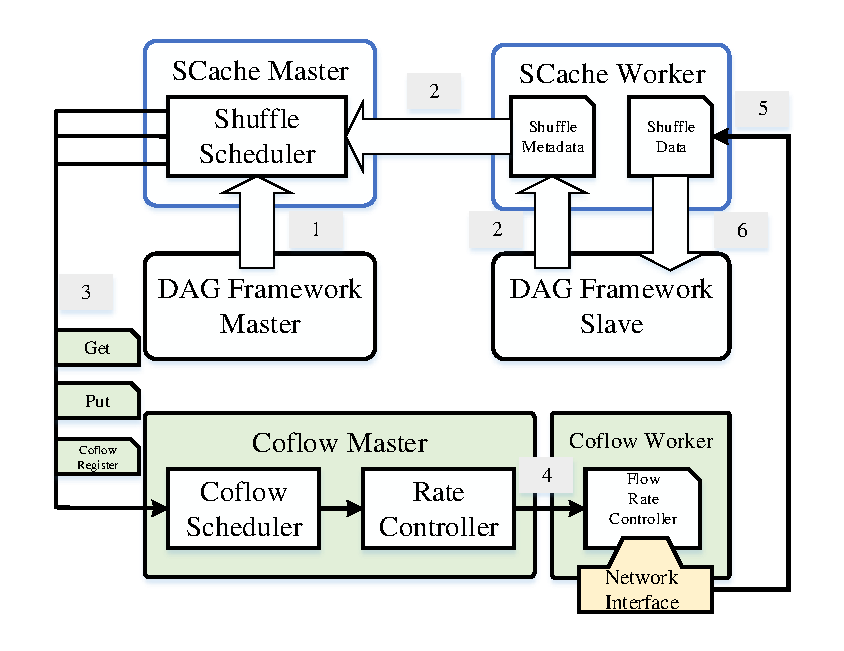
\includegraphics[width=0.85\textwidth]{../figure/coflow.pdf}
	\bicaption[fig:coflow]{SCache结合Coflow调度系统的工作示意图}{SCache结合Coflow调度系统的工作示意图}{Fig}{SCache Works with Coflow Scheduling System}
\end{figure}

对于优化shuffle网络传输这个特定过程,在coflow的层面来看就是最小化coflow的平均传输时间(average \textbf{C}oflow \textbf{C}ompletion \textbf{T}ime,average CCT)。
结合coflow的API列表\ref{tab:coflow}和coflow的这些属性,一个shuffle对应的网络流传输在coflow的优化下需要经过如下步骤:
\begin{enumerate}
	\item 通过driver调用create接口向coflow调度系统注册该shuffle对应的coflow,此时driver会返回一个与该coflow唯一对应的handle,在具体实现中可以是一个唯一的ID。
	该ID会通过广播的形式通知各个工作节点。
	\item 当shuffle中的某个数据块生成完成,对应的工作节点会通过put接口向coflow调度系统放置该流。
	\item 当shuffle中的某个数据块的接收节点可以开始接收该数据块,比如reduce任务已经启动,会通过get接口向coflow调度系统请求该网络流。
	\item 当coflow调度系统收到该coflow中某个流的put和get消息之后,就会更新其对应的节点信息和体积信息等,并且标记为该flow已经可以传输。
	\item 当一个coflow中的所有流都已经被标记为可以传输,coflow调度系统就会根据特定的算法对该coflow进行调度,得出其中每个flow的传输速度,并且开始传输。
	比较典型的coflow之间的调度算法有最小瓶颈coflow优先(Smallest-Effective-Bottleneck-First,SEBF)\cite{varys},而coflow内部的流之间的调度算法有满足最小资源分配算法(Minimum-Allocation-for-
	Desired-Duration,MADD)\cite{varys}等。
\end{enumerate}

从上述的执行流程中可以看到目前coflow的优化是具有一定滞后性的,即需要等到一个shuffle中所有数据块都已经生成并且可以开始传输,在此基础上才能获取完整的coflow信息(比如$length$,$size$等),然后开始调度。
因而目前coflow对于shuffle的优化往往也都停留在离线过程,即所有的流信息都是已知的情况下(Varys\cite{varys},Aalo\cite{aalo},Seagull\cite{seagull}等)才能取得较好的效果。
论文CODA\cite{coda}提出了采用机器学习算法和延迟绑定的策略来缓解coflow信息未知对调度带来的滞后性影响,但是在预测过程中仍然存在5\%的错误率,这些错误的存在可能造成流对coflow的从属关系发生错误,进而影响性能。

而本研究提出的SCache正好能为coflow调度系统提供这些缺失的信息。
对于coflow中每个流的体积,可以通过在map初始阶段对shuffle输出数据分布的预测来获取。
与此同时,coflow中每个流的源节点和目的节点也可以通过启发式的reduce任务预调度获得。
因此在map初始阶段,通过结合本研究的优化策略获取的相关信息便可以通过相应的coflow接口提供给coflow调度系统,从而避免了现有系统的滞后性,获得更好的在线调度性能。

图\ref{fig:coflow}展示了SCache结合典型的集中式coflow调度系统之后,与分布式DAG计算协同完成shuffle的过程示意图。
其具体工作流程主要由以下步骤组成:

\begin{enumerate}
	\item SCache在DAG生成阶段获取shuffle的依赖。
	\item 在map初始阶段,SCache从分布式DAG框架工作节点的任务执行过程中已经完成的shuffle输出数据进行收集。
	之后SCache的主节点根据注册的shuffle依赖与收集的shuffle相关数据进行最终shuffle输出数据分布的预测和reduce任务预调度。
	\item 完成预调度之后,SCache通过create接口向coflow调度系统注册,获取coflow ID。
	根据此ID,将预测过程中每个shuffle数据块的体积作为该coflow中网络流体积。
	map任务执行节点作为流的源节点,预调度的reduce任务执行节点作为目的节点,然后分别调用coflow的put与get接口上传coflow相关的flow信息。
	\item Coflow调度系统主节点收到这些信息后,即可算出相应的coflow调度所需的所有属性,并对该coflow进行优先级调度,同时对其中的每个网络流进行限速。完成调度后,coflow调度系统中心节点将调度信息发送到工作节点。
	\item Coflow工作节点根据接收到的限速信息,在SCache从节点通过本地网卡读取shufffle数据时,对其进行限速。
	\item SCache工作节点将传输完成的shuffle数据通过内存拷贝提供给DAG计算框架的工作进程。
\end{enumerate}

在以上所有工作步骤中,涉及到coflow相关注册与限速的步骤从原先的5个步骤缩短到3个步骤(步骤3,4,5)。
因此通过利用SCache提供的精确的应用层信息,可以大大简化目前coflow调度系统的复杂程度,很好的消除了原先coflow调度系统的滞后性。
更重要的是,SCache提供的信息与coflow调度所需要的信息完美的匹配,能够实现更精确的coflow在线调度,从而进一步优化shuffle在网络传输过程中的开销。

